%% ============================================================================
%% Paper 3: Supplementary Material
%% Target: Journal of Cheminformatics
%% Updated: July 2026
%% ============================================================================

\documentclass[11pt,a4paper]{article}

% Page layout
\usepackage[a4paper,margin=2.5cm]{geometry}

% Fonts and encoding
\usepackage[T1]{fontenc}
\usepackage[utf8]{inputenc}
\usepackage{lmodern}

% Mathematics
\usepackage{amsmath, amsfonts, amssymb, mathtools}

% Figures and tables
\usepackage{graphicx}
\usepackage{booktabs, tabularx, array, longtable}
\usepackage[table]{xcolor}

% Units and SI
\usepackage[
  detect-all           = true,
  group-minimum-digits = 4,
  per-mode             = symbol,
  range-phrase         = {--},
  range-units          = single,
]{siunitx}

% Hyperlinks
\usepackage[authoryear,round]{natbib}
\usepackage[hypertexnames=false,colorlinks=true,linkcolor=blue,citecolor=blue,urlcolor=blue]{hyperref}

% Cross-referencing
\usepackage{cleveref}
\crefname{table}{Table}{Tables}
\Crefname{table}{Table}{Tables}
\crefname{figure}{Figure}{Figures}
\Crefname{figure}{Figure}{Figures}

% Supplementary figure numbering (Figure S1, S2, ...)
\renewcommand{\thefigure}{S\arabic{figure}}
\renewcommand{\thetable}{S\arabic{table}}

% Author information
\usepackage{authblk}

% Caption styling
\usepackage[labelfont=bf,textfont={footnotesize,it}]{caption}

% Path configuration
\graphicspath{{Graphics/}}

% ============================================================================
% AUTHOR INFORMATION
% ============================================================================

\title{\textbf{Supplementary Material}\\Persistent homology resolves the scaffold paradox in AI-generated African antimalarial candidates: a topological and tensor-network fingerprinting study}

\author[1]{Myke Vital Sao Temgoua}
\author[1]{Jean-Pierre Tchapet Njafa}
\author[1]{Serge Guy Nana Engo}
\author[2]{Penabei Samafou}
\author[3]{Wilfred Fon Mbacham}

\affil[1]{Department of Physics, Faculty of Science, University of Yaound\'e I, P.O. Box 812, Yaound\'e, Cameroon}
\affil[2]{Department of Medical Imaging and Radiation Sciences, Universit\'e de Sherbrooke, Sherbrooke, QC, Canada}
\affil[3]{Department of Biochemistry, Faculty of Science, University of Yaound\'e I, P.O. Box 812, Yaound\'e, Cameroon}

\date{\today}

% ============================================================================
% BEGIN DOCUMENT
% ============================================================================

\begin{document}

\maketitle

% ============================================================================
% 1. CROSS-PAPER H$_1$ PERSISTENCE VS. RESISTANCE RESILIENCE SCORE
% ============================================================================

\section{Cross-paper validation: topological persistence and resistance resilience}

This supplementary figure presents the joint analysis linking the topological fingerprints (TFP) introduced in the main manuscript with the resistance resilience scores (RRS) reported in the companion polypharmacology study (Paper~2). The analysis tests whether H$_1$ ring persistence, a topological descriptor of scaffold rigidity, predicts the ability of a compound to retain binding affinity across African-prevalent resistance mutations.

\begin{figure}[htbp]
\centering

\includegraphics[width=0.85\textwidth]{h1_rrs_class_violin.png}
\caption{Joint topological analysis linking Paper~3 TFP features with Paper~2 resistance classification. Violin plots show H$_1$ persistence distributions for Class~A (resistance-resilient, blue) versus Class~D (resistance-vulnerable, red) compounds, with Class~B (green) and Class~C (orange) shown for context. Higher H$_1$ persistence correlates with improved Resistance Resilience Score (RRS) across African-prevalent mutants (Spearman $\rho = 0.947$, permutation $p < 0.0001$, 95\% bootstrap CI $[0.799, 1.000]$, $n = 14$), providing a topological predictor of mutation tolerance without additional MD simulation.}
\label{fig:h1_rrs}
\end{figure}

\section*{Data Availability}

All data supporting the main manuscript and this Supplementary Material are publicly available on Zenodo (DOI: \url{https://doi.org/10.5281/zenodo.19608875}) and mirrored at \url{https://github.com/NanaEngo/Malaria_codesV2} under the MIT licence. See the main manuscript for a full inventory of deposit components.

% ============================================================================

% 2. TOPOLOGICAL FINGERPRINT STATISTICS

% ============================================================================



\section{Topological fingerprint statistics}



Detailed topological fingerprint statistics for the full library are provided in \cref{tab:tda_stats}, and representative persistence diagrams are shown in \cref{fig:persistence}.



\begin{table}[htbp]
\centering
\caption{Topological fingerprint statistics across \num{19836} valid molecules.}
\label{tab:tda_stats}
\begin{tabularx}{\textwidth}{l S[table-format=1.4] S[table-format=1.4] S[table-format=1.4] S[table-format=1.4]}
\toprule
Feature & {Mean} & {Std} & {Min} & {Max} \\
\midrule
H$_0$ entropy & 3.5781 & 0.2014 & 2.2887 & 4.1943 \\
H$_0$ count & 38.0452 & 7.3462 & 11.0000 & 69.0000 \\
H$_0$ max persistence (\si{\angstrom}) & 2.7171 & 0.6725 & 1.9857 & 5.9491 \\
H$_0$ mean persistence (\si{\angstrom}) & 1.6140 & 0.0632 & 1.4414 & 2.0281 \\
\midrule
H$_1$ entropy & 1.6357 & 0.3350 & -0.0000 & 2.7234 \\
H$_1$ count & 3.6058 & 1.3431 & 1.0000 & 10.0000 \\
H$_1$ max persistence (\si{\angstrom}) & 1.3918 & 0.0573 & 0.6238 & 2.7075 \\
H$_1$ mean persistence (\si{\angstrom}) & 0.6136 & 0.1339 & 0.2356 & 1.4000 \\
\midrule
H$_2$ entropy & 0.6956 & 0.3527 & -0.0000 & 1.9579 \\
H$_2$ count & 0.0291 & 0.1691 & 0.0000 & 2.0000 \\
H$_2$ max persistence (\si{\angstrom}) & 0.4669 & 0.0490 & 0.0000 & 1.0522 \\
H$_2$ mean persistence (\si{\angstrom}) & 0.3841 & 0.0885 & 0.0000 & 0.7344 \\
\bottomrule
\end{tabularx}
\end{table}



\begin{figure}[htbp]
\centering
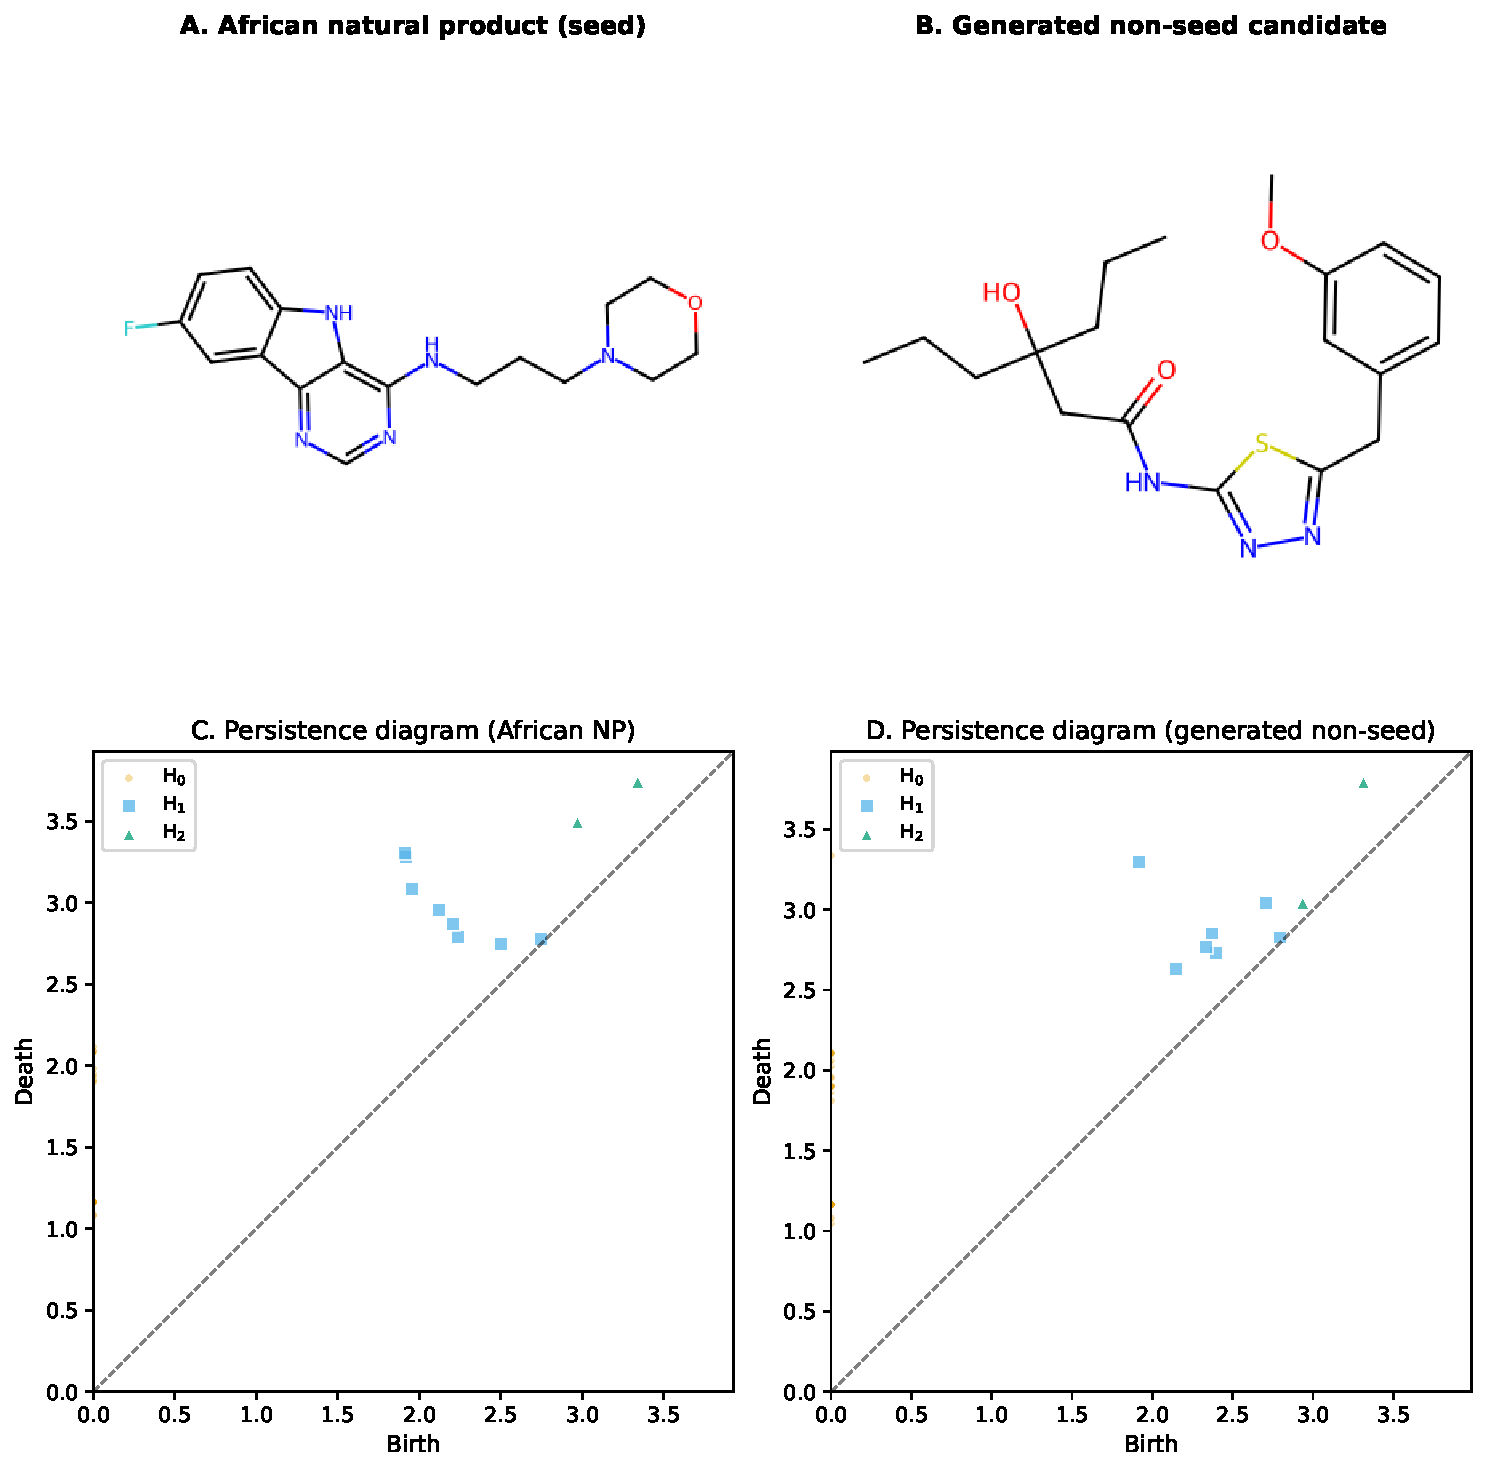
\includegraphics[width=0.75\textwidth]{persistence_diagrams.pdf}
\caption{Representative persistence diagrams for an African natural product and a synthetic drug. Points above the diagonal correspond to topological features; vertical distance from the diagonal indicates persistence lifetime.}
\label{fig:persistence}
\end{figure}



% ============================================================================

% 3. CLUSTERING QUALITY METRICS

% ============================================================================



\section{Clustering quality metrics}



\cref{tab:clustering} reports the clustering quality metrics used to address reviewer question R8.



\begin{table}[htbp]
\centering
\caption{Clustering quality metrics for TNE embeddings versus VAE latent space and ECFP4 fingerprints (KMeans, $k = 484$). Higher Silhouette coefficient indicates better cluster coherence.}
\label{tab:clustering}
\begin{tabularx}{\textwidth}{l S[table-format=1.3]}
\toprule
Descriptor & {Silhouette} \\
\midrule
TNE ($d=8$, \num{192}-dim) & 0.350 \\
VAE latent (\num{64}-dim) & 0.229 \\
ECFP4 (\num{2048}-dim) & 0.180 \\
\bottomrule
\end{tabularx}
\end{table}



% ============================================================================

% 4. GA-STYLE DISCRIMINATOR BENCHMARK

% ============================================================================



\section{GA-style discriminator benchmark}



The full GA-style discriminator benchmark is reported in \cref{tab:ga_discriminator} and visualised in \cref{fig:ga_discriminator}.



\begin{table}[htbp]
\centering
\caption{Chemical similarity vs. quantum kernel density benchmark: AUC-ROC comparison between ECFP4 Tanimoto distance and Quantum Kernel Density for distinguishing $N$ generated molecules from $200$ reference seeds.}
\label{tab:ga_discriminator}
\begin{tabularx}{\textwidth}{l S[table-format=1.4] S[table-format=1.4] S[table-format=-1.4]}
\toprule
{$N$\ generated} & {AUC$_{\text{Tanimoto}}$} & {AUC$_{\text{QK}}$} & {$\Delta$AUC} \\
\midrule
50 & 1.0000 & 0.4252 & -0.5748 \\
100 & 1.0000 & 0.4811 & -0.5189 \\
200 & 1.0000 & 0.4755 & -0.5245 \\
500 & 1.0000 & 0.5114 & -0.4886 \\
\bottomrule
\end{tabularx}
\end{table}



\begin{figure}[htbp]
\centering
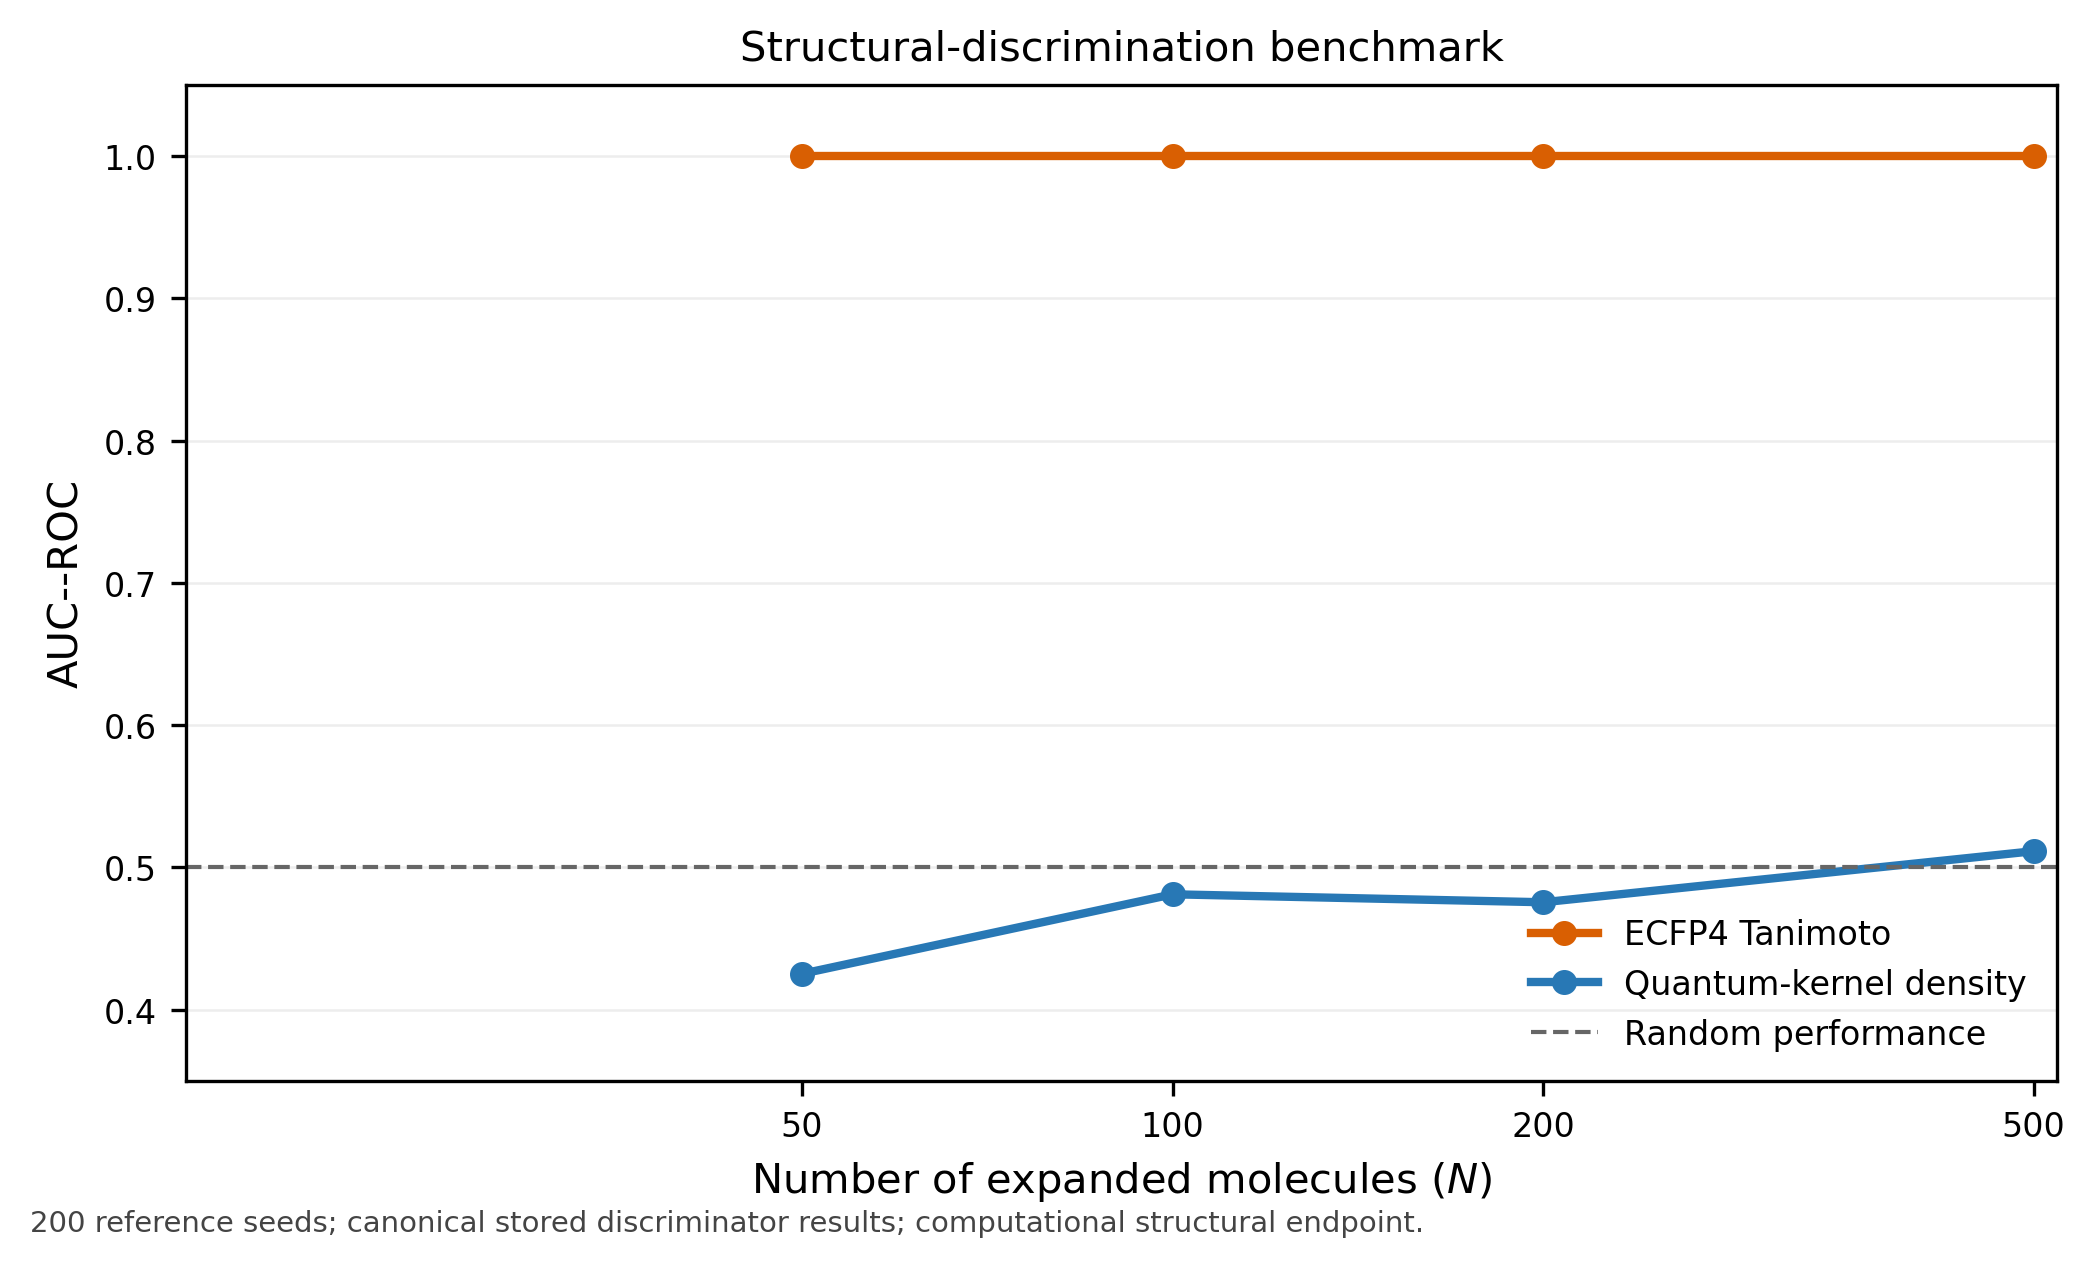
\includegraphics[width=0.80\textwidth]{p3_ga_discriminator.png}
\caption{Chemical similarity vs. quantum kernel density discriminator benchmark. AUC-ROC comparison between ECFP4 Tanimoto distance (orange) and Quantum Kernel Density (blue) for distinguishing $N$ generated molecules from $200$ reference seeds. The dashed grey line marks random performance (AUC = 0.5). ECFP4 achieves perfect discrimination (AUC = 1.0) at all $N$, while the quantum kernel remains near-random (AUC = 0.425--0.511).}
\label{fig:ga_discriminator}
\end{figure}

\end{document}
